\subsection{Video-out Port}
\label{sec:video_out}

The \systemName~includes a video-out port with a VGA controller that can be
connected to a standard VGA monitor. The VGA controller supports a screen resolution of
640 $\times$ 480. The image that is displayed by the VGA controller is
derived from two sources: a {\it pixel} buffer, and a {\it character} buffer.

\subsubsection{Pixel Buffer}
\label{sec:pixel_buffer}

The pixel buffer for the video-out port holds the data (color) for each pixel that is 
displayed by the VGA controller.  As illustrated in Figure \ref{fig:video_coord}, the
pixel buffer provides an image resolution of 
320 $\times$ 240 pixels, with the coordinate 0,0 being at the top-left corner of the image. 
Since the VGA controller supports the screen resolution of 640 $\times$ 480, each of the
pixel values in
the pixel buffer is replicated in both the {\it x} and {\it y} dimensions when it is being
displayed on the VGA screen.

\begin{figure}[h!]
   \begin{center}
       \includegraphics{../../../common/figs/Media_FPGA_Video_Coord.pdf}
   \end{center}
   \caption{Pixel buffer coordinates.}
	\label{fig:video_coord}
\end{figure}

Figure \ref{fig:pixels}$a$ shows that each pixel color is represented as a 16-bit halfword, 
with five bits for the blue and red 
components, and six bits for green.  As depicted in part $b$ of Figure \ref{fig:pixels}, 
pixels are addressed in the pixel buffer by 
using the combination of a {\it base} address and an {\it x,y} offset.  In the \systemName~the default address of the pixel buffer is {\sf 0x\baseAddressOffset 8000000}, which corresponds
to the starting address of the FPGA on-chip memory.  Using this scheme, the pixel at 
location 0,0 has the address {\sf 0x\baseAddressOffset 8000000}, 
the pixel 1,0 has the address {\it base} $+$ (00000000~000000001~0)$_2$ = {\sf 0x\baseAddressOffset 8000002}, 
the pixel 0,1 has the address {\it base} $+$ (00000001~000000000~0)$_2$ = {\sf 0x\baseAddressOffset 8000400}, and 
the pixel at location 319,239 has the address {\it base} $+$ (11101111 100111111 0)$_2$ = 
{\sf 0x\baseAddressOffset 803BE7E}. 

\begin{figure}[h!]
   \begin{center}
       \includegraphics{../../../common/figs/Media_FPGA_Video_Pixels.pdf}
   \end{center}
   \caption{Pixel values and addresses.}
	\label{fig:pixels}
\end{figure}

You can create an image by writing color values into the pixel addresses as described
above. A dedicated {\it pixel buffer controller} continuously reads this pixel 
data from sequential addresses in the corresponding
memory for display on the VGA screen.  You can modify the pixel data at any time, simply
by writing to the pixel addresses. Thus, an image can be changed even when it is in the
process of being displayed.  However, it is also possible to avoid making changes to 
the pixel buffer while it is being displayed, by using the concept of {\it
double-buffering}.  In this scheme, two pixel buffers are involved, called the {\it front} 
and {\it back} buffers, described below.

\subsubsection{Double Buffering}
\label{sec:double_buffer}

As mentioned above, a pixel buffer controller reads data out of the pixel buffer so that it 
can be displayed on the VGA screen. This pixel buffer controller 
includes a programming interface in the form of a set of registers, as
illustrated in Figure~\ref{fig:pixel_ctrl}. The register at address {\sf 0xFF203020} is called 
the {\it Buffer} register, and the register at address  {\sf 0xFF203024} is the 
{\it Backbuffer} register. Each of these registers stores the starting address of a pixel 
buffer.  The Buffer register holds the address of the pixel buffer that is displayed on
the VGA screen. As mentioned above, in the default configuration of the \systemName~this 
Buffer register is set to the address {\sf 0x\baseAddressOffset 8000000}, which points to the start of the FPGA 
on-chip memory.  The default value of the Backbuffer register is also {\sf 0x\baseAddressOffset 8000000},
which means that there is only one pixel buffer. But software can modify the address
stored in the Backbuffer register, thereby creating a second pixel buffer. The pixel
buffer can be located in the SDRAM memory in the \systemName, which has 
the base address {\sf 0x\baseAddressOffset 0000000}. An image can be drawn into the second buffer by writing to its pixel addresses.
This image is not displayed on the VGA monitor until a pixel buffer {\it swap} is performed, 
as explained below.

A pixel buffer swap is caused by writing the value 1 to the Buffer register. This write
operation does not directly modify the content of the Buffer register, but instead causes
the contents of the Buffer and Backbuffer registers to be swapped. The swap operation does
not happen right away; it occurs at the end of a VGA screen-drawing cycle, after the last 
pixel in the bottom-right corner has been displayed. This time instance is referred to as
the {\it vertical synchronization} time, and occurs every 1/60 seconds. Software can poll the
value of the $S$ bit in the {\it Status} register, at address {\sf 0xFF20302C}, to see when 
the vertical synchronization has happened. Writing the value 1 into the Buffer register
causes $S$ to be set to 1. Then, when the swap of the Buffer and Backbuffer registers 
has been completed $S$ is reset back to 0.  

\begin{figure}[h!]
   \begin{center}
       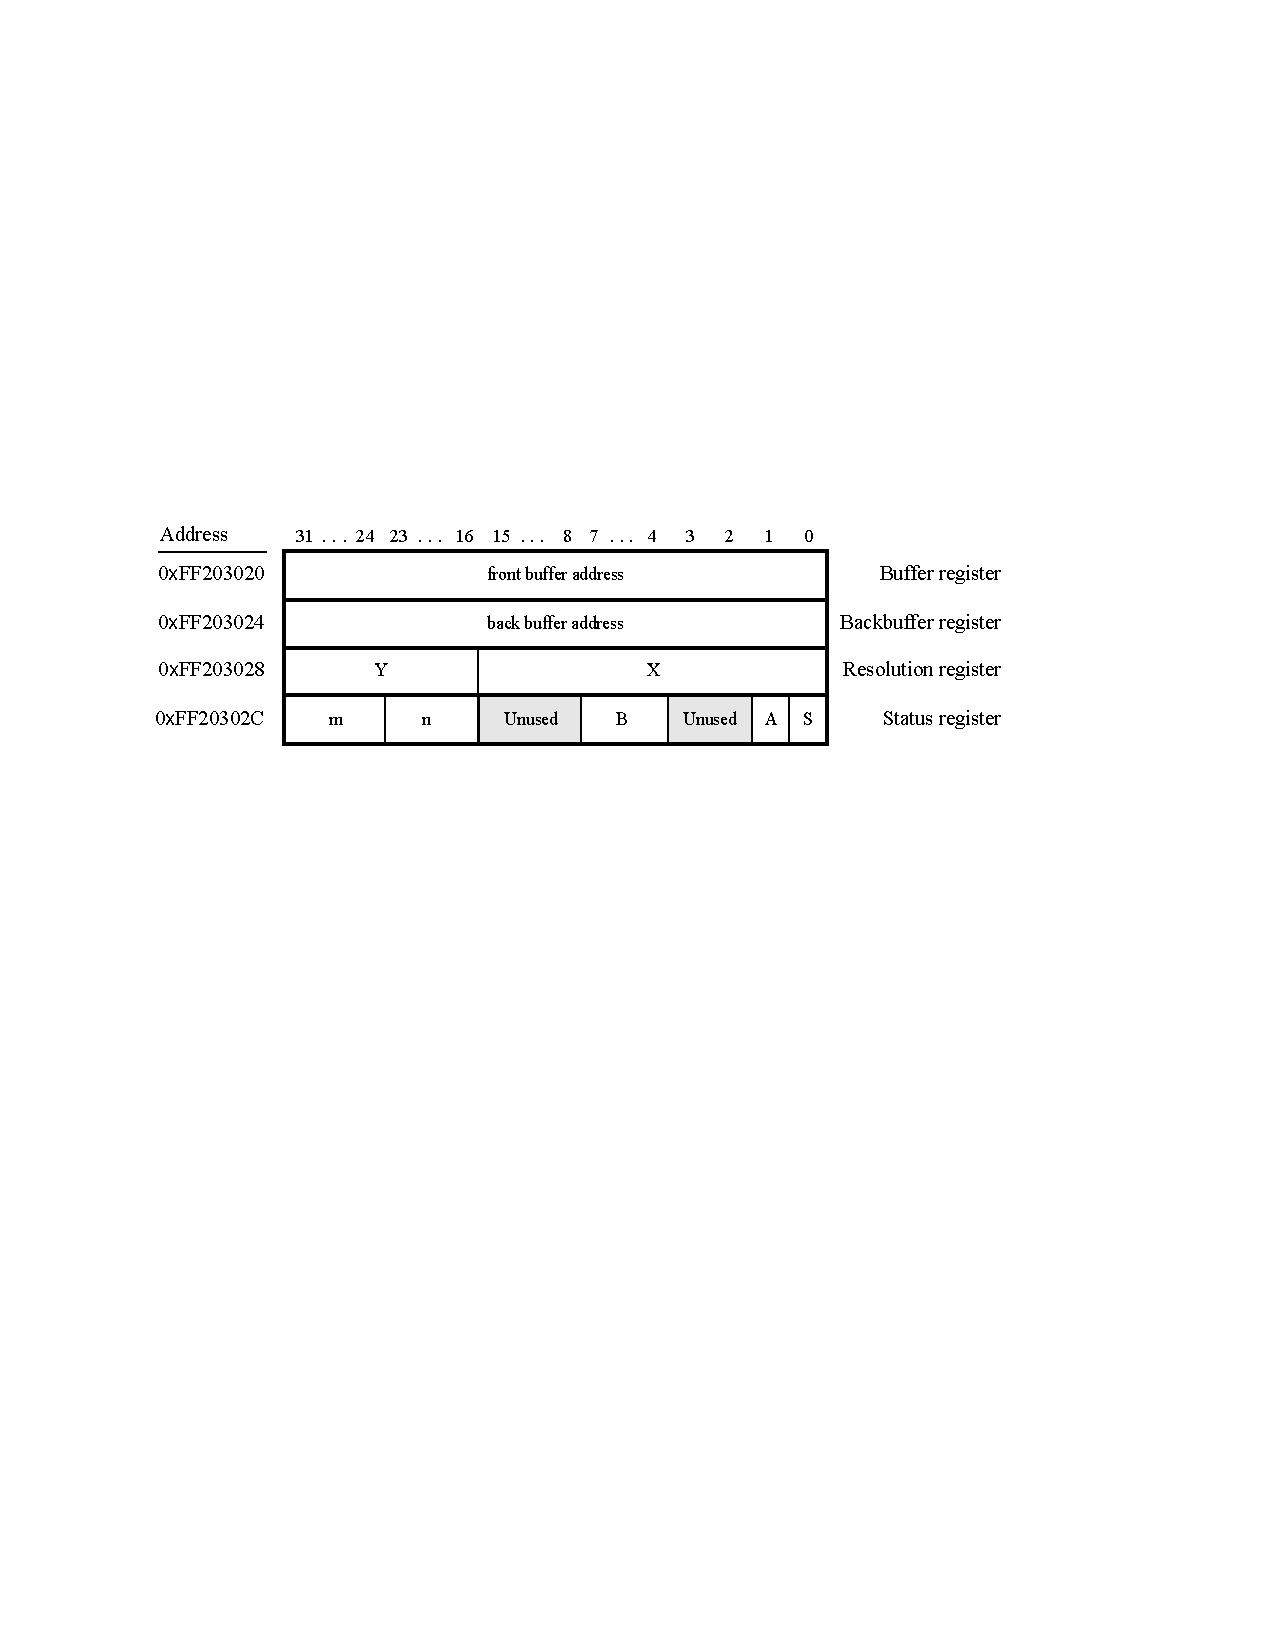
\includegraphics{../../../common/figs/Media_FPGA_Video_Port.pdf}
   \end{center}
   \caption{Pixel buffer controller registers.}
	\label{fig:pixel_ctrl}
\end{figure}

In a typical application the pixel buffer controller is used as follows. While the image
contained in the pixel buffer that is pointed to by the Buffer register is being displayed, 
a new image is drawn into the pixel buffer pointed to by the Backbuffer register. When this new
image is ready to be displayed, a pixel buffer swap is performed. Then, the pixel buffer 
that is now pointed to by the Backbuffer register, which was already displayed, is cleared and 
the next new image is drawn. In this way, the next image to be displayed is always drawn in
the ``back'' pixel buffer, and the two pixel buffer pointers are swapped when the new image 
is ready to be displayed. Each time a swap is performed software has to synchronize with
the VGA controller by waiting until the $S$ bit in the Status register becomes 0.

As shown in Figure~\ref{fig:pixel_ctrl} the {\it Status} register contains additional information
other than the $S$ bit. The fields $n$ and $m$ give the number of address bits used for
the $X$ and $Y$ pixel coordinates, respectively. The $B$ field specifies the number of
bytes used for each pixel, with the minimum being 1 and the maximum 4. The $A$ field allows 
the selection of two different ways of forming pixel addresses. If configured with $A=0$, then 
the pixel controller expects addresses to contain $X$ and $Y$ fields, as we have used in this
section. But if $A=1$, then the controller expects addresses to be consecutive
values starting from 0 and ending at the total number of pixels$ - 1$.

In Figure \ref{fig:pixels}$b$ the default values of the status register fields in the \systemName~are used when forming pixel addresses. The defaults are $n=9$,  $m=8$, $B = 2$,
and $A = 0$. If the pixel buffer controller is changed to provide different values of
these fields, then the way in which pixel addresses are formed has to be modified accordingly. 
The programming interface also includes a {\it Resolution} register, shown 
in Figure~\ref{fig:pixel_ctrl}, that contains the X and Y resolution of the pixel buffer(s).  

\subsubsection{Character Buffer}

The character buffer for the video-out port is stored in on-chip memory in the FPGA
on the \DEBoard~board. As illustrated in Figure \ref{fig:chars}$a$, the buffer provides 
a resolution of 80 $\times$ 60 characters, where each character occupies an 8 $\times$ 8
block of pixels on the VGA screen. Characters are stored in each of the locations shown in
Figure \ref{fig:chars}$a$ using their ASCII codes; when these character codes are 
displayed on the VGA monitor, the character buffer automatically generates the
corresponding pattern of pixels for each character using a built-in font. 
Part $b$ of Figure \ref{fig:chars} shows that characters are addressed in the memory by 
using the combination of a {\it base} address, which has the value 
{\sf 0x\baseAddressOffset 9000000}, and an {\it x,y}
offset. Using this scheme, the character at location 0,0 has the address
{\sf 0x\baseAddressOffset 9000000}, 
the character 1,0 has the address {\it base} $+$ (000000 0000001)$_2$ = {\sf 0x\baseAddressOffset 9000001}, 
the character 0,1 has the address {\it base} $+$ (000001 0000000)$_2$ = {\sf 0x\baseAddressOffset 9000080}, and 
the character at location 79,59 has the address {\it base} $+$ (111011 1001111)$_2$ = 
{\sf 0x\baseAddressOffset 9001DCF}. 

\begin{figure}[h!]
   \begin{center}
       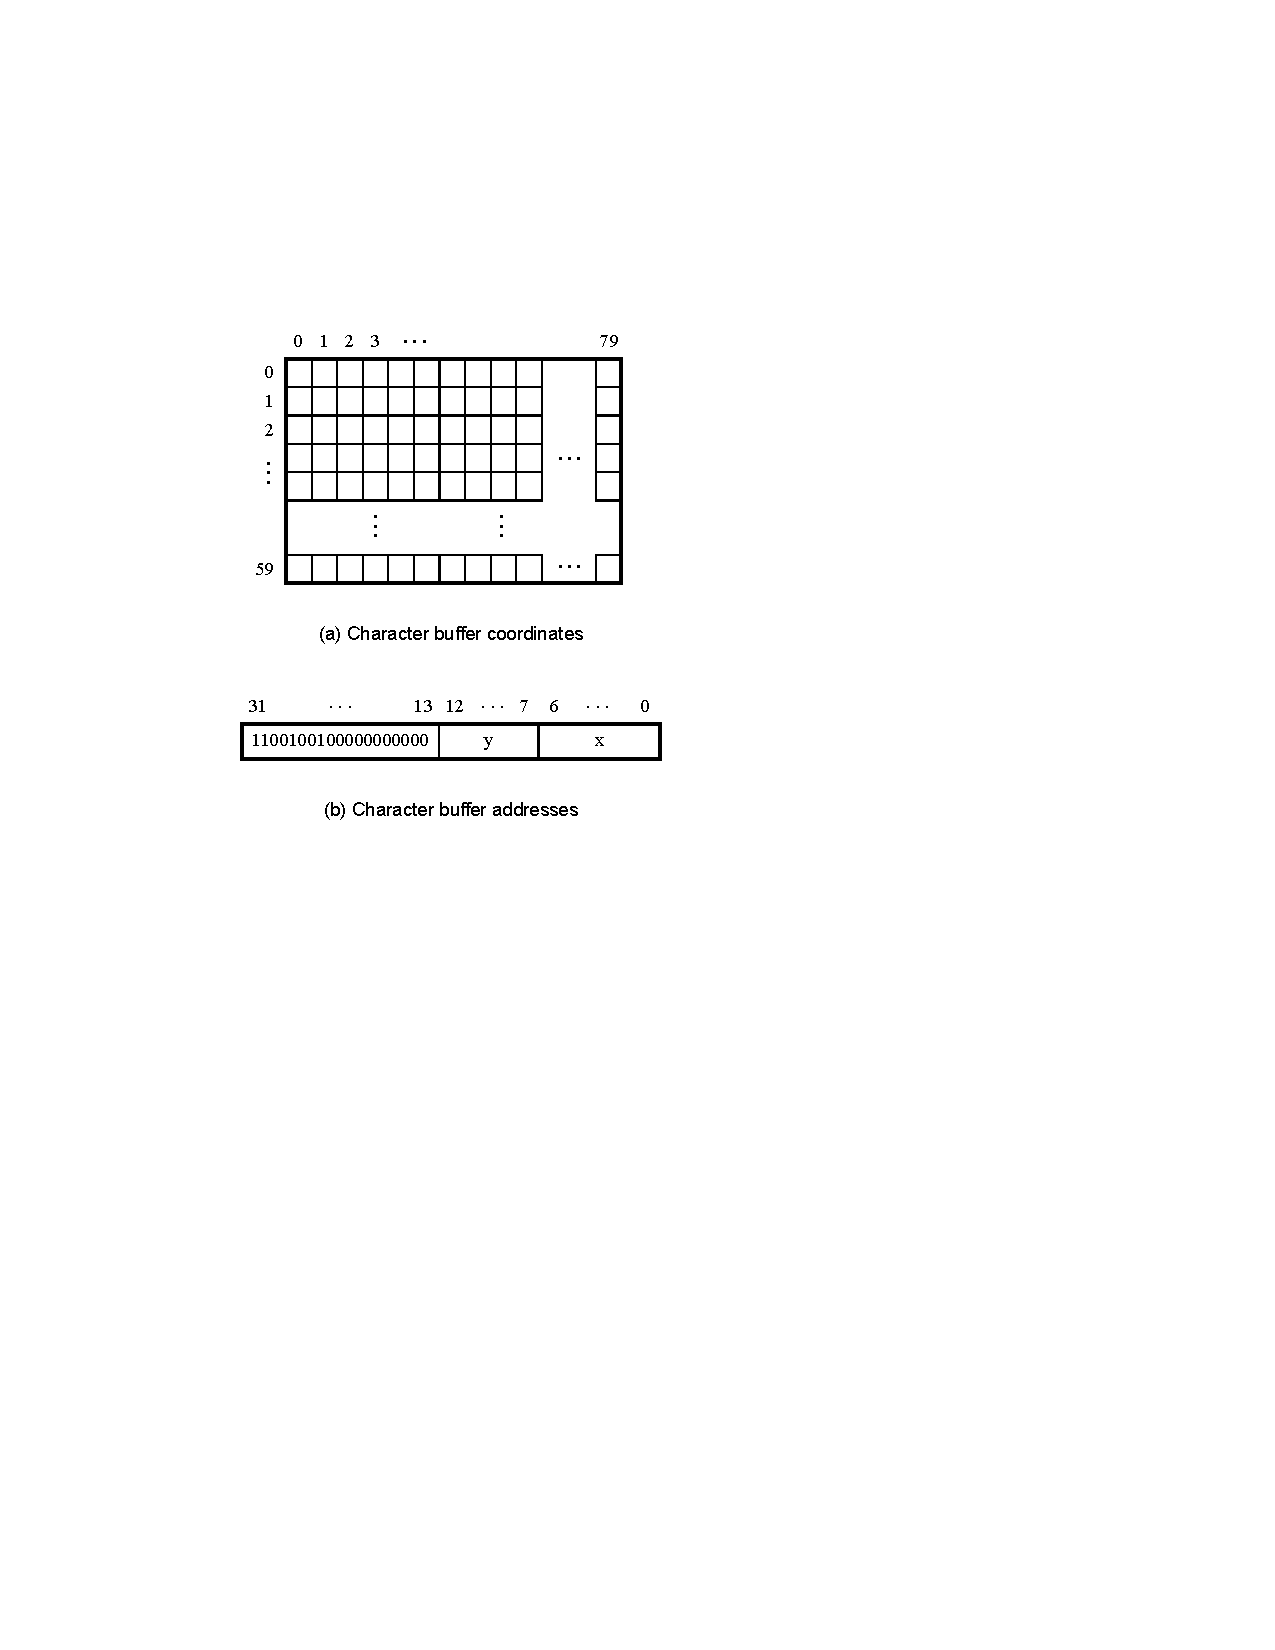
\includegraphics{../../../common/figs/Media_FPGA_Video_Chars.pdf}
   \end{center}
   \caption{Character buffer coordinates and addresses.}
	\label{fig:chars}
\end{figure}

\subsubsection{Using the Video-out Port with C code}

A fragment of C code that uses the pixel and character buffers is shown in 
Figure \ref{fig:video_C}.  The first {\bf for} loop in the figure draws a rectangle in 
the pixel buffer using the color {\it pixel\_color}. The rectangle is drawn using the
coordinates $x_1, y_1$ and $x_2, y_2$.  The second {\bf while} loop in the 
figure writes a null-terminated character
string pointed to by the variable {\it text\_ptr} into the character buffer at the
coordinates {\it x}, {\it y}.  The code in Figure \ref{fig:video_C}
is included in the sample program called {\it Media} that is 
distributed with the \productNameMed{}. 


\begin{figure}[h!]
\begin{center}
\begin{minipage}[t]{12.5 cm}
\begin{tabbing}
ZZZ\=ZZ\=ZZ\=*(pixel\_buffer + offset) = pixel\_color;ZZZZZZZ\= \kill
{\bf volatile} {\bf short} * pixel\_buffer = ({\bf short} *) 0x08000000;\>\>\>\>// Pixel buffer\\
{\bf volatile} {\bf char} * character\_buffer = ({\bf char} *) 0x09000000;\>\>\>\>// Character buffer\\
{\bf int} x1, {\bf int} y1, {\bf int} x2, {\bf int} y2, {\bf short} pixel\_color;\\
{\bf int} offset, row, col;\\
{\bf int} x, {\bf int} y, {\bf char} * text\_ptr;\\
$\ldots$\\
/* Draw a box; assume that the coordinates are valid */\\
{\bf for} (row = y1; row $<$= y2; row++)\\
ZZZ\=ZZ\=ZZ\=*(pixel\_buffer + offset) = pixel\_color;ZZZZZZZ\= \kill
\>{\bf for} (col = x1; col <= x2; ++col)\\
\>\{\\
\>\>offset = (row $<<$ 9) + col;\\
\>\>*(pixel\_buffer + offset) = pixel\_color;	\>\>// compute halfword address, set pixel\\
\>\}\\
\\
/* Display a text string; assume that it fits on one line */\\
offset = (y $<<$ 7) + x;\\
{\bf while} ( *(text\_ptr) )\\
\{\\
\>*(character\_buffer + offset) = *(text\_ptr);	\>\>\>// write to the character buffer\\
\>++text\_ptr;\\
\>++offset;\\
\}\rule{6.0in}{0in}~\\
\end{tabbing}
\end{minipage}
\end{center}
	\vspace{-0.33in}\caption{An example of code that uses the video-out port.}
   \label{fig:video_C}
\end{figure}


